In the Heat Transfer~(HT) algorithm, we have a graph where heat values are
exchanged between nodes. The program stops when, for every node $i$, the new heat values $H_i$
differ only a small $\epsilon$ from the old values $H_{i-1}$, where $\delta =
|H_i - H_{i-1}| \le \epsilon$. The algorithm works asynchronously, i.e., heat
values are updated using information as it arrives from neighboring nodes. This
increases concurrency since nodes do not need to synchronize between
iterations.

Figure~\ref{code:coord:ht} shows the HT rules that send new heat values to
neighbor nodes. In the first rule we added a \code{add-priority} action fact to
increase the priority of the neighbor nodes for the case when the current node
has a large $\delta$. The idea is to prioritize the computation of heat values
of nodes (using \code{update}) that have a neighbor that changed significantly.
Multiple \code{add-priority} facts will increase the priority of a node so that
nodes with multiple large deltas will have higher priority.

\begin{figure}[h!]
\begin{LineCode}[commandchars=\\\[\]]
new-heat(A, New, Old),
fabs(New - Old) > epsilon
   -o {B | !edge(A, B) -o
         new-neighbor-heat(B, A, New),
         update(B), \underline[add-priority(B, Delta)]}.

new-heat(A, New, Old)
fabs(New - Old) <= epsilon
   -o {B | !edge(A, B) -o
         new-neighbor-heat(B, A, New)}.
\end{LineCode}
  \mycap{Coordination code for the Heat Transfer program.}
  \label{code:coord:ht}
\end{figure}

Fig.~\ref{fig:coordination:results_ht} presents the scalability results for the
regular and coordinated version. The dataset used in the experiments was already
used in Section~\ref{section:implementation:performance}, which is a square
grid with an inner square with high heat nodes. Comparing the coordinated
version with the regular version, with 1 thread there is a 50\% reduction in run
time, while for 32 threads there is, on average, a 15\% reduction. The
increasing number of threads makes selecting the higher priority nodes less
likely since each thread is only able to select the higher priority node from
its own (ever decreasing) subgraph.

\begin{figure}[]
        \centering
        \begin{subfigure}[b]{\plotsize\textwidth}
           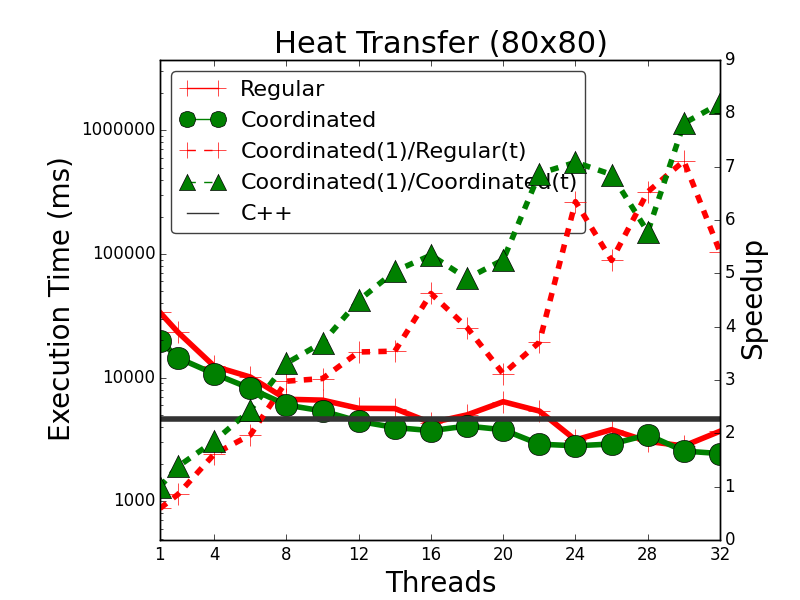
\includegraphics[width=\textwidth]{experiments/coordination/cmp-new-heat-transfer-80.png}
           \label{fig:coordination:coord_ht_80}
           \mycap{80x80 grid dataset.}
        \end{subfigure}
        ~
        \begin{subfigure}[b]{\plotsize\textwidth}
           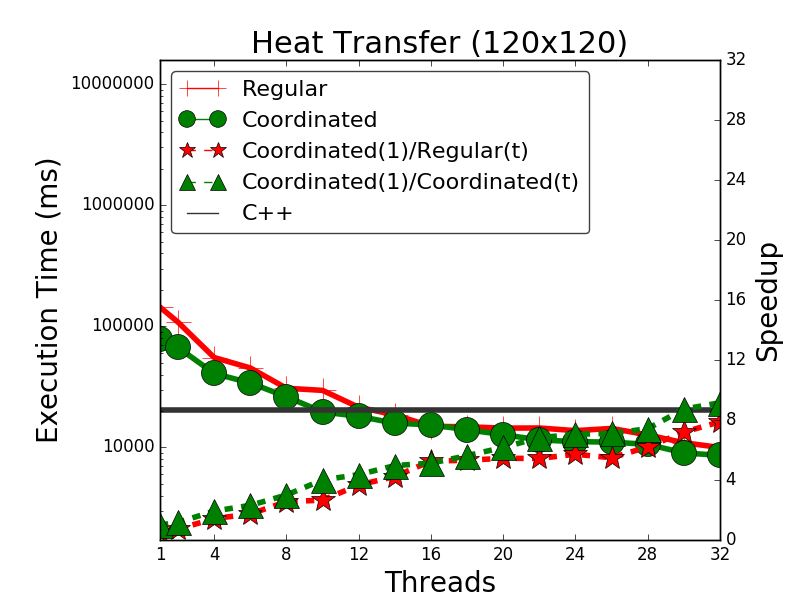
\includegraphics[width=\textwidth]{experiments/coordination/cmp-new-heat-transfer-120.png}
           \label{fig:coordination:coord_ht_120}
           \mycap{120x120 grid dataset.}
        \end{subfigure} \\
        \mycap{Scalability for the Heat Transfer program when using
        coordination. We used the datasets used in
        Section~\ref{section:implementation:performance}}
        \label{fig:coordination:results_ht}
\end{figure}


To further improve locality, we modified the second rule to avoid sending small
$\delta$ values if the target node is in another thread
(Fig.~\ref{code:coord:ht_better}). We use \code{thread-id} to retrieve the
thread \code{T} of the node \code{A} and match the \code{thread-id} of each
neighbor \code{B} against \code{T}. The comprehension in
lines~\ref{line:coord:ht_better_comp1}-\ref{line:coord:ht_better_comp2} only
generates \code{new-neighbor-heat} facts if \code{B} is in the same thread.

The results for the improved version are presented in
Fig.~\ref{fig:coordination:results_ht_new}. There is a clear improvement when
compared to the previous version, since when using 32 threads, there is a 25\%
run time reduction for the coordinated version. For the same number of threads,
the line \textbf{Regular(1)/Coordinated(t)} reaches only a 20-fold speedup,
while the old version reaches a 16-fold speedup. However, this comes at the
price of reduced accuracy in the computed heat values.

\begin{figure}[h!]
\begin{LineCode}[commandchars=\\\[\]]
new-heat(A, New, Old),
fabs(New - Old) > epsilon
   -o {B | !edge(A, B) -o
         new-neighbor-heat(B, A, New),
         update(B), \underline[add-priority(B, Delta)]}.

new-heat(A, New, Old)
fabs(New - Old) <= epsilon,
\underline[thread-id(A, T)]
   -o {B, T | !edge(A, B), \underline[thread-id(B, T)] -o\label[line:coord:ht_better_comp1]
         new-neighbor-heat(B, A, New), \underline[thread-id(B, T)]},\label[line:coord:ht_better_comp2]
      \underline[thread-id(A, T)].
\end{LineCode}

  \mycap{To improve locality, we add an extra constraint to the second rule to
     avoid sending small $\delta$ values if the target node is in another thread.}
  \label{code:coord:ht_better}
\end{figure}

\begin{figure}[]
        \centering
        \begin{subfigure}[b]{\plotsize\textwidth}
           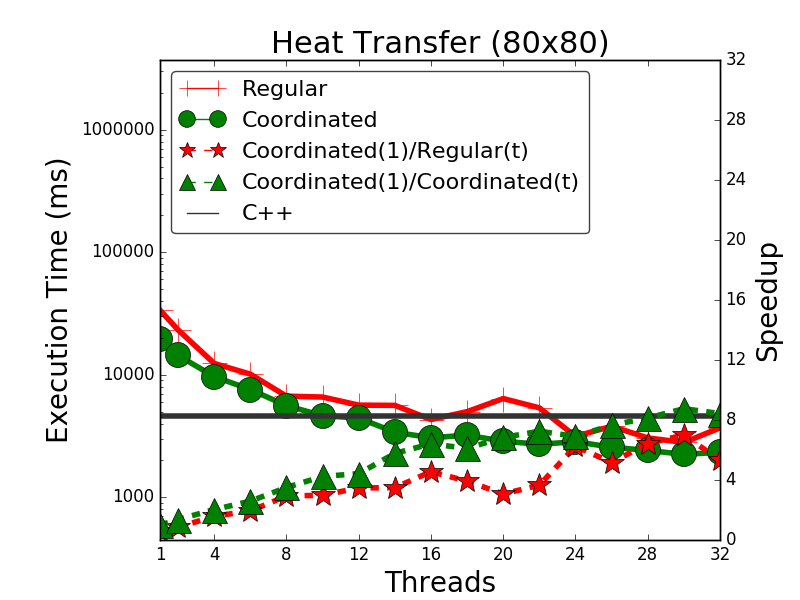
\includegraphics[width=\textwidth]{experiments/coordination/cmpnew-new-heat-transfer-80.png}
           \label{fig:coordination:coord_ht_80}
           \mycap{80x80 grid dataset.}
        \end{subfigure}
        ~
        \begin{subfigure}[b]{\plotsize\textwidth}
           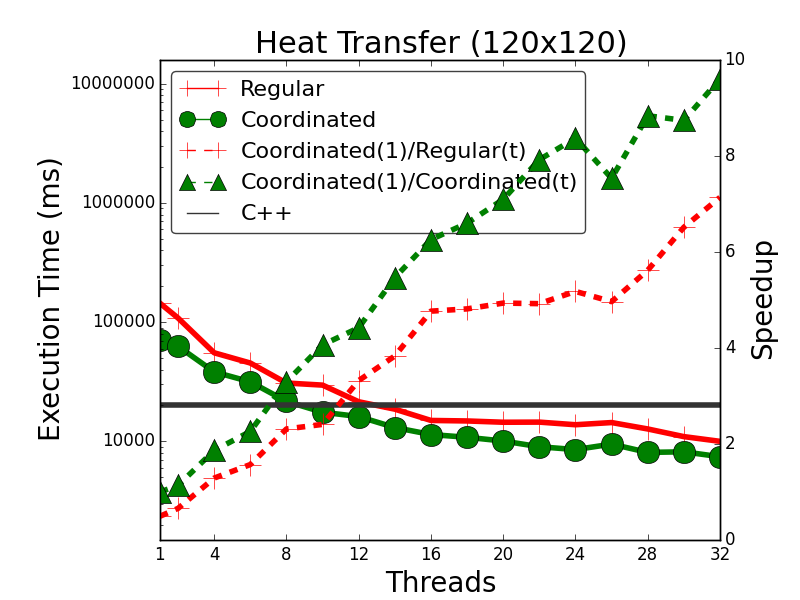
\includegraphics[width=\textwidth]{experiments/coordination/cmpnew-new-heat-transfer-120.png}
           \label{fig:coordination:coord_ht_120}
           \mycap{120x120 grid dataset.}
        \end{subfigure} \\
        \mycap{Scalability for the Heat Transfer program when using
        coordination and avoiding some communication between nodes of different
        threads.}
        \label{fig:coordination:results_ht_new}
\end{figure}
